\chapter{Dataset and Preprocessing}
\label{chap:dataset-preprocessing}

The goal of this stage is to transform raw scalp EEG recordings into a structured
set of seizure-centred windows suitable for functional connectivity estimation
and graph-theoretic analysis. The pipeline is designed to be reproducible and
modular: the dataset is first screened according to explicit eligibility
criteria, raw EEG recordings are then preprocessed, standardized temporal
windows are extracted around seizure onset, and each window is divided into
short epochs. The resulting arrays are used as input for the connectivity
computation described in \cref{chap:connectivity-graph-features}.

\section{CHB-MIT Dataset}
\label{sec:chbmit-dataset}

The experimental work presented in this thesis is based on the CHB-MIT Scalp
EEG Database, a publicly available dataset distributed through PhysioNet and
widely used in seizure detection and seizure prediction research
\cite{PhysioNet-chbmit-1.0.0}. The dataset contains long-term scalp EEG
recordings acquired from pediatric patients with intractable epilepsy during
clinical monitoring. The recordings provide a valuable resource for studying
the temporal evolution of brain activity before and during epileptic seizures.

A note on terminology is necessary because the CHB-MIT dataset distinguishes
between subjects and cases. According to the official PhysioNet description,
the database consists of \num{23} cases obtained from \num{22} pediatric
subjects, since case \texttt{chb21} corresponds to a later recording session of
the same individual as \texttt{chb01}. However, the downloadable dataset used
in this thesis contains case folders ranging from \texttt{chb01} to
\texttt{chb24}. The additional case \texttt{chb24} was added after the original
release and is not included in the \texttt{SUBJECT-INFO} metadata file. For
consistency, the terms \emph{subject}, \emph{case}, and \emph{subject ID} are
used throughout the remainder of this thesis to refer to the CHB-MIT dataset
identifiers rather than necessarily to unique biological individuals.

The EEG recordings are stored in European Data Format (EDF) files, while
seizure onset and offset times are provided through accompanying annotation
files and metadata. These annotations enable a seizure-centred analysis, since
they allow temporal windows to be defined relative to seizure onset and make it
possible to investigate changes in brain dynamics during the preictal period.

The present work adopts a sensor-level approach to functional brain network
analysis. Each bipolar EEG channel is treated as a node in a functional
network, whereas pairwise functional connectivity estimates define weighted
edges between nodes. This approach avoids the need for source reconstruction,
which would require subject-specific anatomical information that is not
available in the CHB-MIT dataset. At the same time, it imposes an important
methodological requirement: network nodes must remain comparable across
subjects, seizures, frequency bands, connectivity measures, and temporal
windows.

To ensure such comparability, a fixed montage consisting of \num{22} bipolar
EEG channels was used throughout the analysis. Maintaining a consistent set of
network nodes is essential for meaningful comparisons of connectivity matrices
and graph-theoretical metrics across recordings. Consequently, only recordings
containing the complete required montage were considered eligible for further
analysis.

\section{Dataset Screening and Eligibility Criteria}
\label{sec:dataset-screening-eligibility}

Not all annotated seizures in the original dataset satisfied the requirements
of the present study. Therefore, a dedicated screening procedure was performed
before preprocessing in order to identify recordings that provided both the
necessary temporal context and the complete channel configuration.

A seizure was retained only if it satisfied two eligibility requirements. First,
at least \SI{540}{\second} of EEG data had to be available before seizure onset.
This corresponds to the \SI{9}{\minute} preictal interval used to extract three
consecutive \SI{3}{\minute} windows before the seizure. Second, the recording
had to contain the complete fixed \num{22}-channel bipolar montage used in this
thesis. Since each channel is later treated as a graph node, missing channels
would produce graphs with different node sets and would make graph metrics
incomparable across seizures.

The overall screening procedure is summarized in
\cref{fig:dataset-screening-flowchart}. The exclusion categories are not
mutually exclusive: some seizures failed both the temporal and channel
requirements.

\begin{figure}[H]
    \centering
    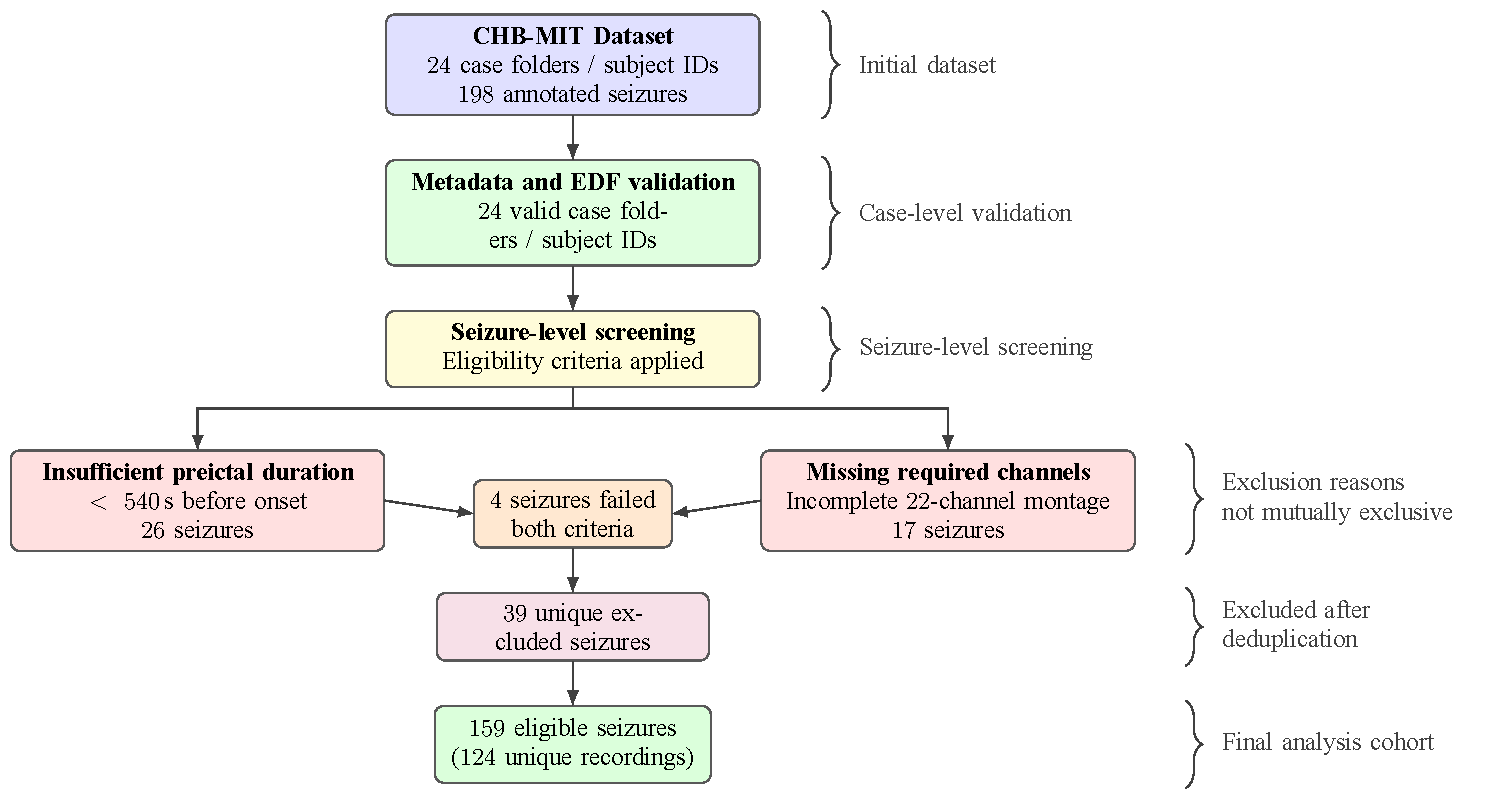
\includegraphics[width=0.95\textwidth]{figures/flowchart.pdf}
    \caption{Flowchart of the dataset screening procedure and seizure eligibility criteria.}
    \label{fig:dataset-screening-flowchart}
\end{figure}

The final screening outcome is reported in
\cref{tab:dataset-screening-summary}. In total, \num{198} annotated seizures
were screened. Of these, \num{159} seizures were retained and \num{39} were
excluded. The retained seizures corresponded to \num{124} unique EEG recordings,
and every screened case folder / subject ID contributed at least one usable
seizure.

\begin{table}[H]
    \centering
    \begin{tabular}{lr}
        \toprule
        Screening quantity & Count \\
        \midrule
        Case folders / subject IDs screened & 24 \\
        Case folders / subject IDs with seizure annotations & 24 \\
        Case folders / subject IDs with readable metadata & 24 \\
        Case folders / subject IDs with at least one usable seizure & 24 \\
        Annotated seizures screened & 198 \\
        Usable seizures retained & 159 \\
        Excluded seizures & 39 \\
        Unique usable recordings & 124 \\
        \bottomrule
    \end{tabular}
    \caption{Summary of dataset screening and seizure eligibility.}
    \label{tab:dataset-screening-summary}
\end{table}

Among the excluded seizures, \num{26} had less than \SI{540}{\second} of
available preictal data and \num{17} were missing one or more channels from the
required bipolar montage. Since \num{4} seizures failed both criteria, the sum
of the individual exclusion reasons is greater than the number of unique
excluded seizures.

The distribution of usable and excluded seizures across case folders is shown
in \cref{fig:subject-vs-seizures-screening}. The figure shows that the dataset
is not balanced across case folders: some contain only a few annotated seizures,
whereas others contain substantially more. This imbalance is important for the
later statistical analysis, because seizures from the same case folder are not
fully independent observations.

\begin{figure}[H]
    \centering
    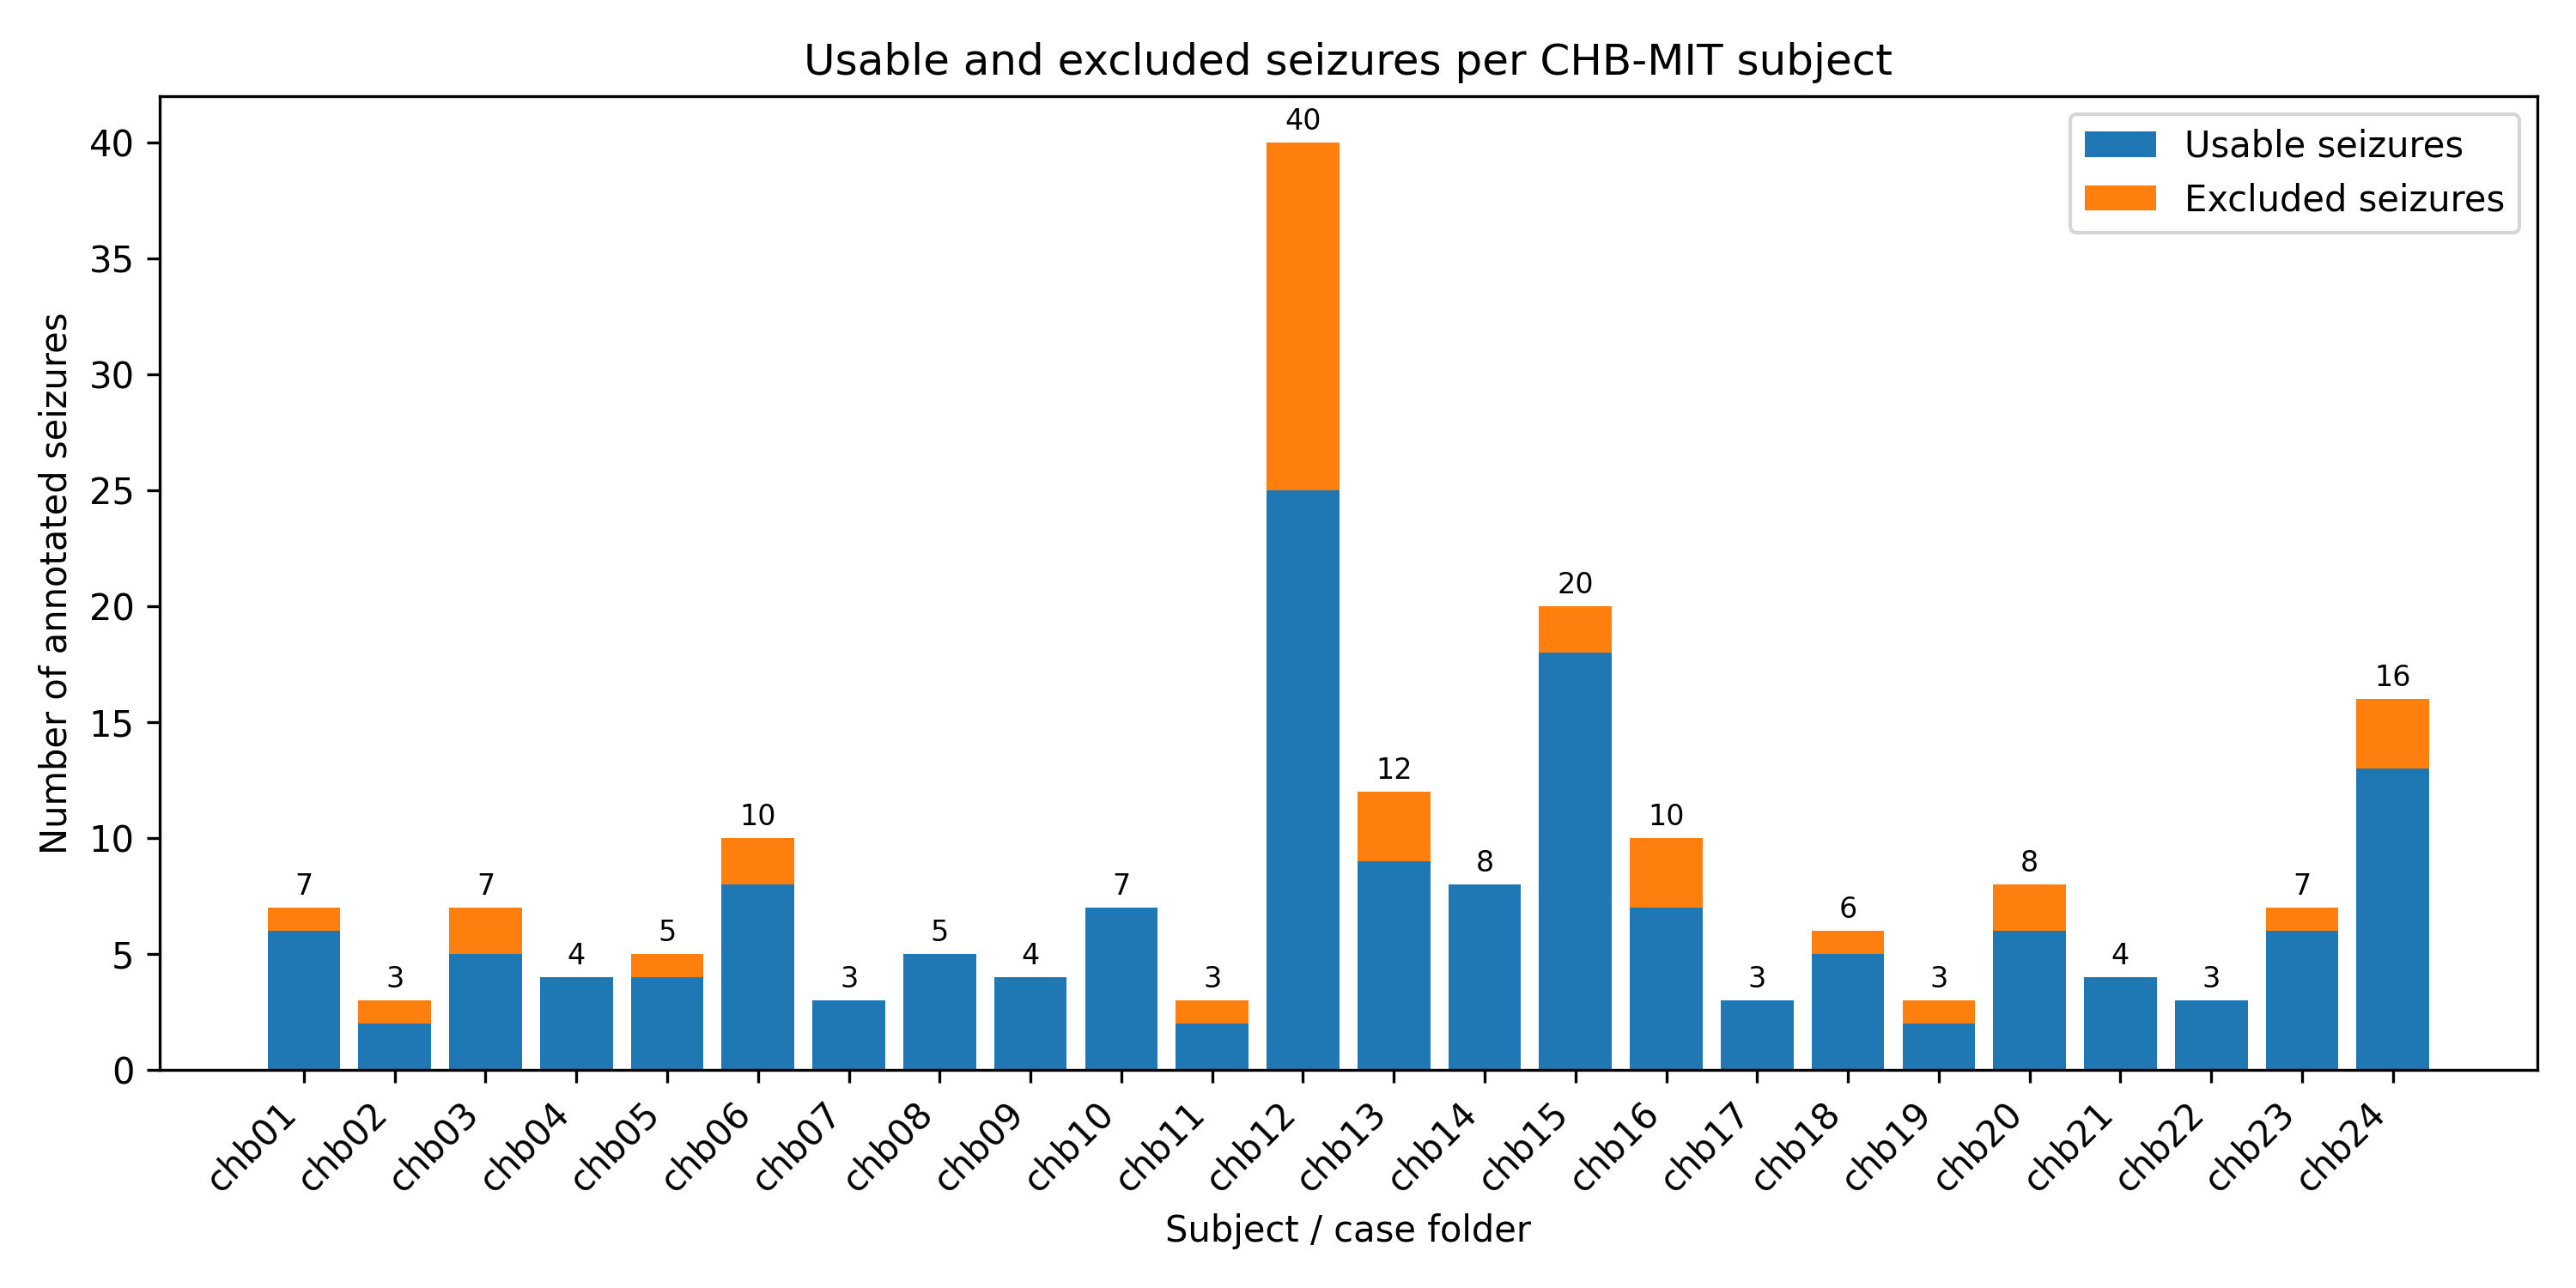
\includegraphics[width=\textwidth]{figures/subject_vs_seizures_screening.png}
    \caption{Number of usable and excluded annotated seizures for each CHB-MIT
    case folder / subject ID after dataset screening. The number above each bar
    indicates the total number of annotated seizures for that case.}
    \label{fig:subject-vs-seizures-screening}
\end{figure}

\section{EEG Preprocessing}
\label{sec:eeg-preprocessing}

After dataset screening, all usable seizure-linked recordings were passed to a
standardized preprocessing pipeline. The purpose of this stage was to transform
the raw EDF recordings into a consistent set of EEG recordings with the same
sampling frequency, channel set, channel order, and filtering characteristics.
This was necessary because the subsequent connectivity and graph-theoretical
analysis requires comparable network nodes across all subjects, seizures, and
time windows.

\subsection{Selection of Recordings for Preprocessing}
\label{subsec:preprocessing-recording-selection}

The preprocessing pipeline used the seizure eligibility table produced during
dataset screening as its input. Only recordings associated with at least one
usable seizure were selected. If multiple usable seizures occurred in the same
EDF recording, the recording was processed only once and reused during the later
segmentation stage. This avoided redundant preprocessing while preserving the
link between each seizure, subject/case folder, and original recording file.

Each selected EDF file was loaded into memory using MNE-Python. The absolute
measurement date stored in the EDF metadata was removed before saving the
processed file, because some CHB-MIT headers contain dates that are outside the
range accepted by the FIF file format. This operation does not affect the
analysis, since all seizure annotations and window definitions in this thesis
are expressed in seconds relative to the beginning of each recording rather than
in absolute calendar time.

\subsection{Channel Selection and Montage Standardization}
\label{subsec:channel-selection-montage-standardization}

A fixed set of \num{22} bipolar EEG channels was retained for all recordings.
These channels define the graph nodes used in the functional connectivity
analysis. The required montage was:

\begin{center}
\begin{tabular}{llll}
\toprule
\texttt{FP1-F7} & \texttt{F7-T7} & \texttt{T7-P7} & \texttt{P7-O1} \\
\texttt{FP1-F3} & \texttt{F3-C3} & \texttt{C3-P3} & \texttt{P3-O1} \\
\texttt{FP2-F4} & \texttt{F4-C4} & \texttt{C4-P4} & \texttt{P4-O2} \\
\texttt{FP2-F8} & \texttt{F8-T8} & \texttt{T8-P8} & \texttt{P8-O2} \\
\texttt{FZ-CZ} & \texttt{CZ-PZ} & \texttt{P7-T7} & \texttt{T7-FT9} \\
\texttt{FT9-FT10} & \texttt{FT10-T8} & & \\
\bottomrule
\end{tabular}
\end{center}

After loading each recording, channel names were normalized to a canonical
format and the recording was checked for the presence of all required channels.
Recordings missing one or more channels from the required bipolar montage were
excluded during dataset screening. Consequently, all recordings retained for
preprocessing contained the complete \num{22}-channel montage.

After validation, the channels were explicitly reordered according to the fixed
montage. This ensured that the same channel index corresponded to the same
bipolar derivation in every preprocessed recording and in every later
connectivity matrix.

\subsection{Handling of Duplicate \texorpdfstring{\texttt{T8-P8}}{T8-P8} Channels}
\label{subsec:t8-p8-duplicate-handling}

Some CHB-MIT recordings contain duplicated versions of the \texttt{T8-P8}
channel. When loaded by MNE-Python, these duplicated channels may appear with
suffixes such as \texttt{T8-P8-0} and \texttt{T8-P8-1}. To preserve a single
canonical version of this bipolar channel, the duplicate channel
\texttt{T8-P8-1} was removed. The retained channel \texttt{T8-P8-0} was then
renamed to the canonical label \texttt{T8-P8}.

This procedure allowed recordings with this naming convention to be retained
while still enforcing the same \num{22}-channel montage across the full
analysis. Importantly, the duplicate channel was handled before the final
channel check and reordering step, so that the output always contained exactly
one \texttt{T8-P8} channel.

\subsection{Sampling Frequency Verification}
\label{subsec:sampling-frequency-verification}

All retained recordings were verified to have a sampling frequency of
\SI{256}{\hertz}. No resampling was applied. Recordings with a mismatched
sampling frequency would have been rejected during preprocessing, but no such
mismatch was observed among the retained usable recordings.

\subsection{Filtering}
\label{subsec:eeg-filtering}
The EEG signals were filtered at the recording level before segmentation. A
finite impulse response (FIR) band-pass filter was applied between
\SI{0.5}{\hertz} and \SI{47}{\hertz}. The lower cutoff was used to attenuate
slow drifts and very low-frequency baseline fluctuations, consistent with
previous quantitative EEG preprocessing approaches in epilepsy research
\cite{Lanzone2022}. The upper cutoff was chosen to match the frequency range
required for the present connectivity analysis and is consistent with the
\SI{47}{\hertz} upper cutoff used by Vecchio et al. in a pre-seizure
graph-theoretical EEG connectivity study \cite{Vecchio2016}.

The highest frequency band analyzed later in the pipeline was the beta2 band
(\SIrange{20}{30}{\hertz}). Therefore, the \SI{47}{\hertz} upper cutoff retained
the full frequency content required for all analyzed bands while suppressing
higher-frequency activity outside the scope of this study. Since the upper
cutoff frequency was below the \SI{60}{\hertz} power-line frequency, no
additional \SI{60}{\hertz} notch filter was applied in the final preprocessing
pipeline.

Filtering was performed on the continuous recording before seizure-centred
windows were extracted. This avoids applying filters separately to short
segments and reduces the risk of introducing window-specific filtering
artifacts.

\subsection{Artifact Handling}
\label{subsec:artifact-handling}

No additional manual or automatic artifact rejection was performed during this
preprocessing stage. This choice was made to keep the preprocessing procedure deterministic and
reproducible across the full dataset. However, it also means that residual
artifacts may still be present in some retained recordings. This limitation is
considered when interpreting the connectivity and graph-theoretical results.

\subsection{Saving Preprocessed Recordings}
\label{subsec:saving-preprocessed-recordings}

After channel standardization, sampling-frequency verification, and filtering,
each preprocessed recording was saved as an intermediate MNE FIF file
and reused during the segmentation stage. Saving these intermediate files
allowed preprocessing to be separated from later analysis steps and ensured that
all subsequent stages used the same standardized recordings.

A preprocessing log was generated to record the processing status of each
selected recording, including the subject/case identifier, recording file,
sampling frequency, number of retained channels, and any error messages.

\section{Temporal Window Definition}
\label{sec:temporal-window-definition}

After preprocessing, seizure-centred temporal windows were extracted from each
eligible seizure recording. The aim of this step was to describe how functional
connectivity and graph-theoretical properties evolve during the minutes
preceding seizure onset. For this reason, the analysis was organized around one
baseline window and three consecutive preictal windows.

The temporal structure was inspired by the design used by Vecchio et al.,
who investigated graph-theoretical changes during the \SI{9}{\minute} period
preceding seizure onset by dividing this interval into three consecutive
\SI{3}{\minute} windows \cite{Vecchio2016}. The present study adopted the same
preictal window structure, but applied it to a larger scalp EEG dataset and to
multiple connectivity measures and graph metrics.

For each seizure, four windows were defined:

\begin{itemize}
    \item \textbf{Baseline}: a \SI{3}{\minute} interictal window selected from
    the same recording, at least \SI{600}{\second} away from any annotated
    seizure activity;
    \item \textbf{T0}: the interval from \SIrange{9}{6}{\minute} before seizure
    onset;
    \item \textbf{T1}: the interval from \SIrange{6}{3}{\minute} before seizure
    onset;
    \item \textbf{T2}: the interval from \SIrange{3}{0}{\minute} before seizure
    onset.
\end{itemize}

The baseline window was used as a reference period representing interictal EEG
activity within the same recording. To reduce contamination by seizure-related
activity, baseline segments were required to be at least \SI{600}{\second}
away from all annotated seizures in that recording. The baseline selection
therefore used all known seizure intervals in the recording, including seizures
that were not retained for the final analysis, because these intervals still
represent ictal periods.

The three preictal windows T0, T1, and T2 covered the final \SI{9}{\minute}
before seizure onset. This organization allowed the analysis to compare
baseline activity with progressively later preictal periods and to examine
whether network properties changed as seizure onset approached. The use of
fixed-duration windows also ensured that connectivity estimates were computed
from equal amounts of data across all seizures and conditions.

Each window had a duration of \SI{180}{\second}. After extraction, each window
was divided into non-overlapping \SI{2}{\second} epochs. Since the sampling
frequency was \SI{256}{\hertz}, each epoch contained \num{512} samples. Thus,
each saved window had the shape

\[
    90 \times 22 \times 512,
\]

corresponding to \num{90} epochs, \num{22} EEG channels, and \num{512} samples
per epoch. These epoch-level representations were then used for the computation
of frequency-specific functional connectivity matrices.

\section{Frequency Band Decomposition}
\label{sec:frequency-band-decomposition}

Functional connectivity was computed separately within predefined EEG frequency
bands. This was done because epileptic brain dynamics may affect different
frequency ranges in different ways, and graph-theoretical properties can depend
on the spectral content used to define the functional network.

The frequency bands used in this thesis followed the band structure adopted by
Vecchio et al. \cite{Vecchio2016}. In particular, the alpha and beta ranges were
subdivided into narrower bands, allowing potential differences between lower and
higher alpha or beta activity to be examined separately. The analyzed frequency
bands were:

\begin{table}[H]
    \centering
    \begin{tabular}{ll}
        \toprule
        Frequency band & Frequency range \\
        \midrule
        Delta & \SIrange{2}{4}{\hertz} \\
        Theta & \SIrange{4}{8}{\hertz} \\
        Alpha1 & \SIrange{8}{10}{\hertz} \\
        Alpha2 & \SIrange{10}{13}{\hertz} \\
        Beta1 & \SIrange{13}{20}{\hertz} \\
        Beta2 & \SIrange{20}{30}{\hertz} \\
        \bottomrule
    \end{tabular}
    \caption{Frequency bands used for functional connectivity analysis.}
    \label{tab:frequency-bands}
\end{table}

Although gamma-band activity is often considered in EEG studies, it was not
included in the present analysis. The frequency decomposition was predefined to
match the study that motivated the temporal and spectral structure of this
work, which focused on delta, theta, alpha, and beta sub-bands. In addition,
gamma-band scalp EEG is more vulnerable to contamination by muscle activity and
other high-frequency artifacts. Since no dedicated artifact rejection procedure
was applied in this pipeline, the analysis was restricted to frequencies up to
the beta2 band, ending at \SI{30}{\hertz}.

This restriction also kept the number of frequency bands and statistical tests
manageable. Gamma-band connectivity is therefore left as a possible extension
for future work rather than being included in the main analysis.